% =============================================================================
%  T-RO extension of "Geometry-Aware Control Barrier Functions for Collision
%  Avoidance via Bernstein Polynomial Approximations" (ICRA 2026, arXiv:2605.30696)
%
%  Numbers come from the scripts in the parent folder:
%     cspace_sdf_cbf_compare.py --scenario switch | dock --steps 700  (Table IV)
%     cspace_cbf_5robots.py                                           (five-robot swap)
%     cspace_experiments.py cache|repr|sens|stats|dock2|unicycle|static|percell
%     make_paper_figs.py overview|dock2|five                          (Figs. 1, 6, 7)
%     dock_shapes.py: ground-truth outlines of the tapered-receptacle docking experiment
%  Raw results: ../results/*.json and ../results/*.log
%
%  Double-anonymous review: \anonymoustrue hides the authors and the running head; the prior
%  conference paper and the ICRA'27 manuscript are cited in the third person and supplied to the
%  editor. Set \anonymousfalse for the final version.
%
%  OPEN ITEMS (kept out of the PDF):
%   - confirm author list/order and affiliations with all co-authors
%   - cover letter: relation to [jo2026geometry] (authors' own) and to [jo2027semantic] (under review)
%   - compile and check the page count (limit: 18 pages for a first submission)
%   - hardware experiment; polytopic / multi-feature closest-point baselines (see Sec. IX)
% =============================================================================
\documentclass[journal]{IEEEtran}

\usepackage{amsmath,amssymb,amsthm}
\usepackage{graphicx}
\usepackage{booktabs}
\usepackage{algorithm}
\usepackage{algpseudocode}
\usepackage{xcolor}
\usepackage{cite}

\newtheorem{theorem}{Theorem}
\newtheorem{lemma}{Lemma}
\newtheorem{proposition}{Proposition}
\newtheorem{corollary}{Corollary}
\newtheorem{assumption}{Assumption}
\theoremstyle{definition}
\newtheorem{definition}{Definition}
\newtheorem{remark}{Remark}

\newcommand{\R}{\mathbb{R}}
\newcommand{\Sone}{\mathbb{S}^1}
\newcommand{\norm}[1]{\left\lVert #1\right\rVert}
\newcommand{\CO}{\mathcal{C}}
\newcommand{\Mset}{\mathcal{M}}
\newcommand{\Rot}{\mathbf{R}}
\DeclareMathOperator{\conv}{conv}
\DeclareMathOperator*{\argmin}{arg\,min}

\graphicspath{{figs/}}

\newif\ifanonymous
\anonymoustrue

\begin{document}

\title{Certified Configuration-Space Distance Fields\\
for Geometry-Aware Control Barrier Functions\\
between Non-Convex Rotating Robots}

\ifanonymous
\author{Anonymous Authors}
\markboth{IEEE Transactions on Robotics}%
{Certified Configuration-Space Distance Fields for Geometry-Aware CBFs}
\else
\author{Siwon~Jo, Yanze~Zhang, Yupeng~Yang, and~Wenhao~Luo%
\thanks{A preliminary version of this work appeared at the IEEE International Conference on
Robotics and Automation (ICRA), 2026~\cite{jo2026geometry}. Section~\ref{sec:relation}
summarizes the differences.}%
\thanks{S.~Jo is with the GRASP Laboratory, University of Pennsylvania, Philadelphia, PA 19104,
USA. Y.~Zhang and W.~Luo are with the Department of Computer Science, University of Illinois
Chicago, Chicago, IL 60607, USA. Y.~Yang is with the Department of Computer Science, University
of North Carolina at Charlotte, Charlotte, NC 28223, USA.}}

\markboth{IEEE Transactions on Robotics}%
{Jo \MakeLowercase{\textit{et al.}}: Certified Configuration-Space Distance Fields for Geometry-Aware CBFs}
\fi

\maketitle

% -----------------------------------------------------------------------------
\begin{abstract}
Control barrier functions (CBFs) are widely used as safety filters for collision avoidance, but
their effectiveness hinges on how geometry is encoded. Geometry-aware CBFs that evaluate signed
distance fields at closest boundary points need convex level sets, treat non-convex geometry only
through rotation-invariant bounding circles, and rely on a heuristic enclosure margin. For every
pair of rigid planar bodies, we represent the configuration-space obstacle over the full relative
pose by one smooth tensor-product B-spline field, so that a single scalar barrier per pair
captures non-convex shapes and rotation without closest points. We show that every first contact
occurs at a configuration built explicitly from the two boundary parametrizations. A Bernstein
branch-and-bound then certifies, for all continuous orientations and without Minkowski sums, that
the barrier is negative at every such configuration; the same machinery certifies its regularity
and the band in which it is switched off. The guarantees hold in exact arithmetic and continuous
time. We also compare global Bernstein polynomials, piecewise B\'ezier patches, and B-splines as
representations. In simulation, the barrier prevented all collisions of non-convex rotating
robots, unlike a closest-point barrier, and enabled docking maneuvers that bounding circles
preclude.
\end{abstract}

\begin{IEEEkeywords}
Collision avoidance, control barrier functions, configuration space, signed distance fields,
B-splines, Bernstein polynomials, multi-robot systems.
\end{IEEEkeywords}

% -----------------------------------------------------------------------------
\section{Introduction}\label{sec:intro}

\IEEEPARstart{S}{afe} navigation depends on how shapes interact across poses rather than on
center-to-center distances. Control barrier functions (CBFs)~\cite{ames2019cbf} turn such safety
conditions into constraints on the control input, typically enforced by a quadratic program (QP)
that minimally modifies a nominal command. Their practical value for collision avoidance, however,
is determined by the geometric surrogate behind the barrier. Spheres and
super-ellipsoids~\cite{wang2017safety,wang2017quadrotors} are smooth and inexpensive but
conservative for irregular shapes. Polytopic formulations are exact for convex pieces but become
pairwise and piecewise in cluttered, non-convex scenes~\cite{chen2025minkowski,thirugnanam2025strongly}.
Learned or non-parametric barriers~\cite{khan2022gaussian,long2021learning} and point-cloud
barriers~\cite{dai2024sailing} trade exactness for generality.

Jo et al.~\cite{jo2026geometry} proposed geometry-aware CBFs
built on Bernstein-polynomial signed distance fields (SDFs)~\cite{li2024representing}: each robot
and the composite obstacle set are represented by smooth SDFs, and the barrier is the robot's SDF
evaluated at the closest point of the obstacle boundary, obtained from the Karush--Kuhn--Tucker
(KKT) conditions. That formulation has three limitations, which this article addresses.
\begin{enumerate}
\item[L1)] \emph{Convexity.} The time derivative of the closest-point barrier relies on the
closest point moving smoothly, which is guaranteed only for convex level sets.
\item[L2)] \emph{Composite and non-convex geometry.} When the closest point jumps between boundary
pieces, the barrier is non-smooth. The work~\cite{jo2026geometry} resorted to a configuration space built
by inflating obstacles with the robot's bounding circle, which ignores orientation and is
conservative precisely for the elongated and non-convex robots that motivate SDFs.
\item[L3)] \emph{Enclosure.} The enclosure of the true geometry by the fitted level set was
enforced with a user-chosen margin, without a certificate.
\end{enumerate}

\begin{figure*}[t]
\centering
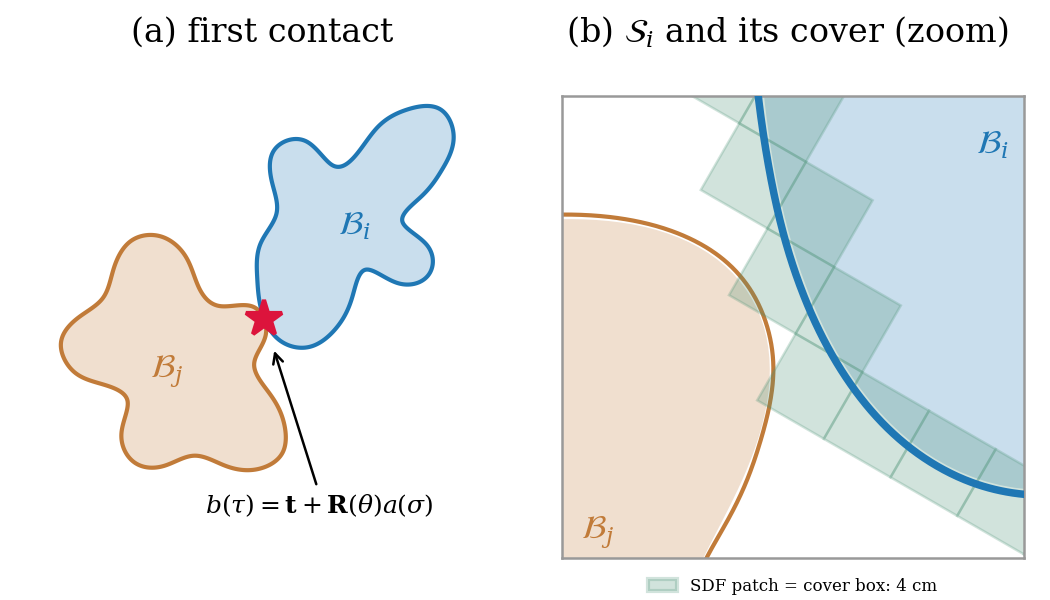
\includegraphics[width=\textwidth]{overview.png}
\caption{Overview. (a) Every first contact between two bodies occurs at a configuration
$\mathbf t=b(\tau)-\Rot(\theta)a(\sigma)$ that joins a boundary point of one body to a boundary
point of the other (Lemma~\ref{lem:contact}). (b) The configuration-space obstacle $\CO_{ij}$ of a
C-shaped and a three-lobed body (black: rasterized reference with 1-cm resolution, eight orientations) and the certified level set
$\{\phi_{ij}=l^\star_{ij}\}$ of a single B-spline field (red). (c) The first-contact set
$\Mset_{ij}$, an explicit three-parameter family; the branch-and-bound of Sec.~\ref{sec:cert}
certifies $\phi_{ij}<l^\star_{ij}$ on all of it, for all continuous orientations.}
\label{fig:overview}
\end{figure*}

\subsection{Approach and Contributions}
We move the SDF from the workspace to the \emph{relative configuration space} of each pair of
bodies, including orientation (Fig.~\ref{fig:overview}). The configuration-space obstacle of a
pair is represented by one smooth tensor-product B-spline field over $(x,y,\theta)$, periodic in
$\theta$, and the barrier is that field minus a certified level. The contributions are as follows.
\begin{enumerate}
\item \emph{Configuration-space SDF CBF over $SE(2)$} (Sec.~\ref{sec:cspace}): one scalar, smooth
barrier per pair of non-convex rotating bodies, with an input-affine derivative when both bodies
move, and with neither closest-point computations nor convexity assumptions (resolves L1 and L2).
\item \emph{Certified first-contact exclusion without Minkowski sums} (Sec.~\ref{sec:cert}): a
first-contact lemma shows that every configuration at which two compact bodies start to touch has
the form $b(\tau)-\Rot(\theta)a(\sigma)$ in terms of their boundary parametrizations. A Bernstein
branch-and-bound over $(\sigma,\tau,\theta)$ certifies a level below which the field stays on all
such configurations, for all continuous orientations; combined with forward invariance, this
implies collision avoidance of the fitted and of the ground-truth shapes from any collision-free
start (resolves L3). The same tools certify the regularity of the barrier and the band in which it
is switched off. The certificates are proved in exact arithmetic; our implementation evaluates them
in double precision without verified rounding bounds.
\item \emph{A Bernstein-form family of representations} (Sec.~\ref{sec:repr}): the global Bernstein
polynomial of~\cite{jo2026geometry}, piecewise B\'ezier patches, and B-splines share cell-wise
Bernstein coefficients, so the same certificate applies to all. The $C^0$ member violates the $C^1$
requirement of CBFs, with visible consequences in closed loop, and the cubic B-spline is an accurate
member that satisfies it.
\item \emph{Evaluation} (Sec.~\ref{sec:exp}) on non-convex rotating robots under single-integrator
and unicycle dynamics, including a docking task, random five-robot swaps against closest-point and
bounding-circle barriers, a robot among many static obstacles, a comparison with adapted
sampling-based and ball-world controllers on shared translation-only geometry, and a sensitivity
analysis of the conservatism with per-cell certified error bounds.
\end{enumerate}

\subsection{Relation to Prior Work}\label{sec:relation}
This article builds on the closest-point formulation of~\cite{jo2026geometry}. It keeps the problem
formulation, the Bernstein-form representation of distance fields, the idea of a single smooth
field that encodes all geometric interaction, the pairwise multi-robot QP, and the experimental
protocol. It replaces the closest-point barrier (retained as a special case and a baseline,
Sec.~\ref{sec:workspace}), the bounding-circle configuration space (now the exact $SE(2)$
configuration space), and the heuristic margin (now a certified level). New are the
configuration-space barrier and its derivative, the first-contact lemma and the collision-avoidance
theorem, the branch-and-bound, band and regularity certificates, the feasibility result, the
representation analysis, and all experiments in Sec.~\ref{sec:exp}. The fitting of body boundaries
with a certified enclosure of the ground truth (Sec.~\ref{sec:cert-body}) and the conversion of
B-splines to Bernstein form follow~\cite{jo2027semantic} and are not claimed as contributions; the
certificate over the three-parameter contact set of a rotating pair is new.

% -----------------------------------------------------------------------------
\section{Related Work}\label{sec:related}

\subsection{Geometric Barrier Functions}
Pairwise barriers between discs or spheres are the standard multi-robot safety
certificates~\cite{wang2017safety}; super-ellipsoids extend them to elongated
vehicles~\cite{wang2017quadrotors}. Both are smooth and inexpensive, but a single primitive
over-approximates irregular or non-convex bodies, and unions of primitives multiply the number of
constraints. For convex polytopes, differentiable signed distances computed through convex programs
in the Minkowski-difference space yield exact barriers~\cite{chen2025minkowski}, and smooth
barriers exist between strongly convex regions~\cite{thirugnanam2025strongly}; non-convex bodies
must then be decomposed, again pairwise per piece. Point-cloud barriers~\cite{dai2024sailing} and
learned or Gaussian-process barriers~\cite{long2021learning,khan2022gaussian} trade exactness for
generality and, in the latter case, online cost. Explicit smooth barriers for polygons avoid
closest points and convex programs by composing edge-wise bounds on the signed distance with smooth
maximum and minimum approximations~\cite{wu2025optimization}; they are tailored to polygons and
trade tightness for smoothness. Exact signed distances between polytopes obtained through Minkowski
operations have recently been combined with nonsmooth CBFs and rotational
gradients~\cite{chen2026exact}, again for convex pieces. For non-convex shapes, sampled distance
functions yield nonsmooth barriers whose sampling error can be quantified~\cite{lutkus2025sampling},
and diffeomorphisms to ball worlds make multiple non-convex unsafe sets amenable to CBFs without
undesired equilibria~\cite{notomista2021nonconvex}; we compare with adaptations of both in
Sec.~\ref{sec:three-baselines}. Jo et al.~\cite{jo2026geometry} built
barriers on Bernstein-polynomial SDFs~\cite{li2024representing} evaluated at closest points. The
present article keeps the smooth-field view but moves it to configuration space, which removes the
closest point and the convexity it requires.

\subsection{Configuration-Space Distance Fields for Control}
Distance fields over the configuration space have been used as barriers for manipulators: neural
configuration-space distance functions serve as CBFs with distributionally robust margins for
learning and sensing errors~\cite{long2025neural}, and differentiable distance fields map obstacle
motion into joint space for time-varying CBFs~\cite{chi2024safe}; see also~\cite{li2024representing}
for workspace distance fields of articulated robots. These works establish configuration-space
distances as useful barriers; they do not certify that the learned or fitted field is below its
level at every configuration where contact can first occur. We address this question for pairs of
rotating non-convex rigid planar bodies: the certificate turns an offline fitted field, trained on
approximate targets, into a single input-affine safety constraint whose correctness does not depend
on the accuracy of those targets.

\subsection{Configuration-Space Obstacles}
Configuration-space obstacles of polygons, with and without rotation, can be constructed
exactly~\cite{lozanoperez1983spatial,latombe1991robot} or on grids through convolution of occupancy
maps~\cite{kavraki1995fft}; such constructions underlie much of motion planning. We do not construct
configuration-space obstacles for safety. We only certify a smooth surrogate against their boundary
through the explicit first-contact parametrization of Lemma~\ref{lem:contact}, and we use a grid
convolution merely to produce training data.

\subsection{Bernstein Bounds and Subdivision}
The convex-hull property of Bernstein and B\'ezier representations and de~Casteljau subdivision
give rigorous and successively tighter bounds on polynomials over
boxes~\cite{farin2002curves,sherbrooke1993computation}. They were used in~\cite{jo2027semantic} to
certify that planar spline boundaries enclose obstacles and to turn polynomial CBF conditions into
finite coefficient constraints. We use the same tools in three variables $(\sigma,\tau,\theta)$ and
on tensor-product fields.

% -----------------------------------------------------------------------------
\section{Preliminaries and Problem Statement}\label{sec:prelim}

\subsection{Control Barrier Functions}
Consider $\dot{\mathbf z}=f(\mathbf z)+g(\mathbf z)\mathbf u$ with $f,g$ locally Lipschitz and
$\mathbf u\in\mathcal U$. For a continuously differentiable $h$, let
$\mathcal H=\{\mathbf z\mid h(\mathbf z)\ge0\}$.

\begin{lemma}[\cite{ames2019cbf}]\label{lem:cbf}
If a locally Lipschitz feedback $\mathbf k(\mathbf z)\in\mathcal U$ satisfies
$L_fh(\mathbf z)+L_gh(\mathbf z)\mathbf k(\mathbf z)\ge-\gamma h(\mathbf z)$ with $\gamma>0$ on an
open set containing $\mathcal H$, then $h(\mathbf z(t))\ge e^{-\gamma t}h(\mathbf z(0))$, and
$\mathcal H$ is forward invariant.
\end{lemma}

\subsection{Bernstein Polynomials and Cubic B-Splines}
The cubic Bernstein basis on $[0,1]$ is $B_r(\xi)=\binom{3}{r}\xi^r(1-\xi)^{3-r}$, $r=0,\dots,3$.
It is nonnegative and sums to one, so a polynomial $p(\xi)=\sum_r\beta_rB_r(\xi)$ satisfies
$\min_r\beta_r\le p(\xi)\le\max_r\beta_r$ (convex-hull property). The same holds for tensor
products $p(\xi,\eta,\zeta)=\sum_{r,s,w}\beta_{rsw}B_r(\xi)B_s(\eta)B_w(\zeta)$.

\emph{Restriction to a sub-interval.} Let $M_B$ map Bernstein to power coefficients,
$p(\xi)=[1,\xi,\xi^2,\xi^3]M_B\boldsymbol\beta$. Substituting $\xi=\xi_0+\Delta v$ gives
$[1,\xi,\xi^2,\xi^3]=[1,v,v^2,v^3]T(\xi_0,\Delta)$ with $T_{jr}=\binom{r}{j}\xi_0^{r-j}\Delta^j$ for
$j\le r$. Hence, the Bernstein coefficients of $p$ restricted to $[\xi_0,\xi_0+\Delta]$ and
reparametrized to $[0,1]$ are
\begin{equation}\label{eq:subdiv}
\boldsymbol\beta'=S(\xi_0,\xi_0+\Delta)\,\boldsymbol\beta,\qquad
S=M_B^{-1}\,T(\xi_0,\Delta)\,M_B .
\end{equation}
In several variables, $S$ acts along each axis. As $\Delta\to0$, the restricted coefficients
converge to the value of $p$, so bounds obtained from~\eqref{eq:subdiv} become tight under
subdivision.

A uniform cubic B-spline with knot spacing $h$ is, on each knot span, a cubic polynomial whose
Bernstein (B\'ezier) coefficients follow from the four active control values
$\mathbf P_{c},\dots,\mathbf P_{c+3}$ through~\cite{farin2002curves,jo2027semantic}
\begin{equation}\label{eq:b2b}
\boldsymbol\beta_c=Q\,[\mathbf P_{c},\mathbf P_{c+1},\mathbf P_{c+2},\mathbf P_{c+3}]^{\top},\quad
Q=\tfrac16\begin{bmatrix}1&4&1&0\\0&4&2&0\\0&2&4&0\\0&1&4&1\end{bmatrix}.
\end{equation}
Tensor products apply $Q$ along each axis.

\subsection{Robots, Relative Configuration, and Problem Statement}
Robot $i\in\{1,\dots,N\}$ is a rigid planar body $\mathcal B_i\subset\R^2$ (compact and connected,
expressed in its body frame, not necessarily convex) with pose $\mathbf x_i=(\mathbf p_i,\theta_i)\in SE(2)$.
Unless stated otherwise, we use $SE(2)$ single-integrator dynamics $\dot{\mathbf p}_i=\mathbf v_i$,
$\dot\theta_i=\omega_i$, $\mathbf u_i=(\mathbf v_i,\omega_i)$, with $\norm{\mathbf v_i}\le v_{\max}$
and $|\omega_i|\le\omega_{\max}$; unicycle robots are treated in Sec.~\ref{sec:unicycle-model}.
Robot $i$ occupies $\Rot(\theta_i)\mathcal B_i+\mathbf p_i$, and we let
$\rho_i=\max_{\mathbf y\in\mathcal B_i}\norm{\mathbf y}$. In the implementation, $\rho_i$ is the
maximum over dense samples of the boundary curve; it only sizes the field domain and guides
subdivision, and no guarantee below depends on its accuracy (see the remark after
Proposition~\ref{prop:bb}).

\begin{definition}[Relative configuration and configuration-space obstacle]
The configuration of robot $i$ relative to robot $j$ is
\begin{equation}\label{eq:qrel}
\mathbf q_{ij}=(\mathbf t_{ij},\theta_{ij}),\quad
\mathbf t_{ij}=\Rot(-\theta_j)(\mathbf p_i-\mathbf p_j),\quad
\theta_{ij}=\theta_i-\theta_j\in\Sone .
\end{equation}
The robots intersect if and only if $\mathbf q_{ij}\in\CO_{ij}$, where
\begin{equation}\label{eq:CO}
\CO_{ij}=\{(\mathbf t,\theta)\in\R^2\times\Sone\mid
(\Rot(\theta)\mathcal B_i+\mathbf t)\cap\mathcal B_j\neq\emptyset\}.
\end{equation}
\end{definition}

\emph{Problem.} Given nominal inputs $\mathbf u^{\rm nom}$, find inputs that minimally modify them
such that no pair of robots ever intersects, for arbitrary (non-convex) compact shapes and with
rotation, using constraints whose number grows with the number of pairs but not with shape
complexity, and whose correctness is certified rather than sampled.

% -----------------------------------------------------------------------------
\section{Closest-Point Workspace Formulation}\label{sec:workspace}
In~\cite{jo2026geometry}, robot $i$ and the obstacles are represented by Bernstein-polynomial SDFs,
the closest obstacle-boundary point $\mathbf p^\star=\argmin_{\mathbf p}F_i(\mathbf x_i,\mathbf p)$
subject to $F_o(\mathbf p)=0$ is computed, and $h=F_i(\mathbf x_i,\mathbf p^\star)$. Its derivative
uses the KKT tangency $\nabla_{\mathbf p}F_i^\top\dot{\mathbf p}^\star=0$, which requires
$\mathbf p^\star$ to move smoothly. This holds for strictly convex level sets but fails when
$\mathbf p^\star$ jumps between separated boundary pieces, as for non-convex bodies or composite
obstacles (L1, L2). The remedy of~\cite{jo2026geometry}, inflating obstacles by the robot's bounding
circle, is a translation-only configuration space; the formulation below replaces it with the exact
$SE(2)$ configuration space.

As a baseline, we retain a direct version of this barrier without a distance field: the signed
distance between the two fitted bodies, $h=d_{ij}-m$, whose derivative at a unique closest pair
$(\mathbf p_a,\mathbf p_b)$ with unit normal $\mathbf n$ is
$\dot h=\mathbf n^\top\big(\mathbf v_i+\omega_iJ(\mathbf p_a-\mathbf p_i)-\mathbf v_j
-\omega_jJ(\mathbf p_b-\mathbf p_j)\big)$, with $J$ as in Proposition~\ref{prop:hdot}. In our
implementation, the fitted boundaries are sampled as polygons with 480--1280 vertices, and one
closest pair is used per step. This removes the field-fitting error of~\cite{jo2026geometry} but
keeps its single-closest-point structure. For non-convex bodies, the closest pair jumps and this
derivative is only one-sided; nonsmooth formulations that account for all active closest features
could mitigate this, and we do not evaluate them.

% -----------------------------------------------------------------------------
\section{Configuration-Space SDF Barrier}\label{sec:cspace}

\subsection{Field and Barrier}
For each unordered pair of shapes, we fit, offline, a field $\phi_{ij}:\Omega_{ij}\to\R$ on
$\Omega_{ij}=[-D_{ij},D_{ij}]^2\times\Sone$ that approximates the signed distance to $\CO_{ij}$ in
$\mathbf t$ (negative inside):
\begin{equation}\label{eq:field}
\phi_{ij}(\mathbf t,\theta)=\sum_{a,b,c}W_{abc}\,N_a(t_x)\,N_b(t_y)\,\tilde N_c(\theta),
\end{equation}
with uniform cubic B-spline bases $N_a,N_b$ and a periodic cubic B-spline basis $\tilde N_c$ in
$\theta$. We take $D_{ij}>\rho_i+\rho_j$; outside $\Omega_{ij}$, the bodies cannot touch because
$\norm{\mathbf t_{ij}}>\rho_i+\rho_j$. Given a certified level $l^\star_{ij}$ (Sec.~\ref{sec:cert}),
the barrier is
\begin{equation}\label{eq:h}
h_{ij}(\mathbf x_i,\mathbf x_j)=\phi_{ij}(\mathbf q_{ij})-l^\star_{ij}.
\end{equation}
Because $\phi_{ij}$ is $C^2$ in all arguments, $h_{ij}$ is $C^2$ whenever $\mathbf q_{ij}$ lies in
the interior of $\Omega_{ij}$. No closest point, projection, or convexity is involved.

\emph{Fitting.} Training targets affect only conservatism, never safety: whatever the fit, the
certificate of Sec.~\ref{sec:cert} determines $l^\star_{ij}$, and a poor fit can only raise it or
make certification fail. Any approximation of the signed distance to $\CO_{ij}$ on a tensor grid of
$(\mathbf t,\theta)$ can therefore be used. We take 96 orientations, rasterize $\CO_{ij}$ at each
with 1-cm resolution by convolving occupancy masks, compute signed distances by Euclidean distance
transforms, and sample them on a $100\times100$ grid per orientation. The fit is a separable ridge
regression, $W=T\times_1M_x\times_2M_y\times_3M_\theta$ with
$M_\ast=(\Phi_\ast^\top\Phi_\ast+\lambda I)^{-1}\Phi_\ast^\top$ per axis and $\lambda=10^{-4}$. We
stress that this discretization is used only to generate training data; the contact certificate
never samples orientations.

\subsection{Time Derivative}
\begin{proposition}\label{prop:hdot}
Let $J=\left[\begin{smallmatrix}0&-1\\1&0\end{smallmatrix}\right]$,
$\mathbf g_t=\nabla_{\mathbf t}\phi_{ij}(\mathbf q_{ij})$, and
$g_\theta=\partial_\theta\phi_{ij}(\mathbf q_{ij})$. Under $SE(2)$ single-integrator dynamics,
\begin{equation}\label{eq:hdot}
\dot h_{ij}=\big(\Rot(\theta_j)\mathbf g_t\big)^{\!\top}(\mathbf v_i-\mathbf v_j)
+g_\theta\,\omega_i-\big(\mathbf g_t^{\top}J\mathbf t_{ij}+g_\theta\big)\omega_j ,
\end{equation}
which is affine in $(\mathbf u_i,\mathbf u_j)$.
\end{proposition}
\begin{proof}
Since $\tfrac{d}{d\alpha}\Rot(\alpha)=\Rot(\alpha)J$ and $J$ commutes with $\Rot$,
$\dot{\mathbf t}_{ij}=-\omega_jJ\mathbf t_{ij}+\Rot(-\theta_j)(\mathbf v_i-\mathbf v_j)$ and
$\dot\theta_{ij}=\omega_i-\omega_j$. The chain rule and
$\mathbf g_t^\top\Rot(-\theta_j)=(\Rot(\theta_j)\mathbf g_t)^\top$ yield~\eqref{eq:hdot}.
\end{proof}

\subsection{Unicycle Robots}\label{sec:unicycle-model}
For $\dot{\mathbf p}_i=v_i\mathbf e(\theta_i)$ and $\dot\theta_i=\omega_i$ with
$\mathbf e(\theta)=[\cos\theta,\sin\theta]^\top$, substituting into~\eqref{eq:hdot} gives
\begin{equation}\label{eq:hdot-uni}
\dot h_{ij}=a_i v_i+g_\theta\omega_i-a_jv_j-\big(\mathbf g_t^\top J\mathbf t_{ij}+g_\theta\big)\omega_j,
\end{equation}
where $a_k=(\Rot(\theta_j)\mathbf g_t)^{\top}\mathbf e(\theta_k)$; the derivative is still affine in
the inputs. The barrier has relative degree one wherever the coefficient vector
$(a_i,g_\theta,-a_j,-\mathbf g_t^\top J\mathbf t_{ij}-g_\theta)$ is nonzero. It vanishes only if both
headings are orthogonal to $\Rot(\theta_j)\mathbf g_t$ and both angular coefficients vanish.
Regularity (Proposition~\ref{prop:reg}) excludes $\nabla\phi_{ij}=0$ but not this alignment, so we
monitor the coefficient norm in the experiments.

\subsection{Multi-Robot Safety Filter}
With $\mathbf u=(\mathbf u_1,\dots,\mathbf u_N)$, the controller is
\begin{equation}\label{eq:qp}
\begin{aligned}
\mathbf u^\ast=\argmin_{\mathbf u}\ &\norm{\mathbf u-\mathbf u^{\rm nom}}^2\\
\text{s.t. }&\dot h_{ij}(\mathbf u)\ge-\gamma h_{ij}\quad\forall (i,j)\in\mathcal A,\\
&\norm{\mathbf v_i}\le v_{\max},\ |\omega_i|\le\omega_{\max}\quad\forall i,
\end{aligned}
\end{equation}
where $\mathcal A$ collects the pairs with $\norm{\mathbf t_{ij}}_\infty<D_{ij}-\delta$. There is one
scalar constraint per active pair, independent of shape complexity. With the speed disc,
\eqref{eq:qp} is a second-order cone program; in our implementation, the disc is replaced by an
inscribed 12-gon, which makes it a QP, solved exactly as a least-distance program via non-negative
least squares~\cite{lawson1995solving} and warm-started by constraint generation (the minimizer of a
relaxation that satisfies all constraints is the minimizer of the full QP).

\begin{proposition}[Feasibility on the safe set]\label{prop:feas}
Under $SE(2)$ single-integrator or unicycle dynamics with a centralized filter~\eqref{eq:qp}, if
$h_{ij}\ge0$ for every active pair, then $\mathbf u=\mathbf 0$ is feasible, with the speed disc or
with any input set that contains the origin.
\end{proposition}
\begin{proof}
The dynamics are driftless, so $\mathbf u=\mathbf 0$ gives $\dot h_{ij}=0\ge-\gamma h_{ij}$ for
all active pairs by~\eqref{eq:hdot} and~\eqref{eq:hdot-uni}, and $\mathbf 0$ satisfies the input
bounds.
\end{proof}
Feasibility on the safe set therefore holds for any number of active pairs. It does not imply goal
convergence (Sec.~\ref{sec:limits}) or local Lipschitz continuity of the minimizer, and it does not
extend to states with $h_{ij}<0$, to dynamics with drift, or to obstacles that move independently of
the filter. In our experiments, a slack variable is added only if~\eqref{eq:qp} is infeasible, which
by Proposition~\ref{prop:feas} can happen only after a discrete-time violation.

\begin{assumption}[Activation band]\label{ass:band}
$h_{ij}>0$ on $\{\mathbf q\in\Omega_{ij}\mid D_{ij}-\delta\le\norm{\mathbf t}_\infty\le D_{ij}\}$.
\end{assumption}
Assumption~\ref{ass:band} makes the activation of a pair harmless: a pair enters $\mathcal A$ with
$h_{ij}>0$. It is verified offline: the minimum Bernstein coefficient of every cell that meets the
band is a lower bound of $\phi_{ij}$ there, and we require it to exceed $l^\star_{ij}$. We use a
fixed band width $\delta=0.125$~m and $D_{ij}=\rho_i+\rho_j+0.3$~m, so that the activation
boundary lies outside the region $\norm{\mathbf t}\le\rho_i+\rho_j$ in which contact is possible;
a band tied to the cell size would violate this for coarse fields.

\begin{remark}[Static obstacles]\label{rem:static}
For a robot among static obstacles $\mathcal O=\bigcup_k\mathcal O_k$, the configuration-space
obstacle of the union is the union of the configuration-space obstacles. One field over the
workspace and $\theta$ therefore encodes all obstacles in a single barrier, retaining the ``one SDF
for many obstacles'' property of~\cite{jo2026geometry} while becoming exact in orientation. The
certificate of Sec.~\ref{sec:cert} applies with $b$ ranging over all obstacle boundaries, and the
online cost is one field evaluation, independent of the number of obstacles
(Sec.~\ref{sec:exp-static}).
\end{remark}

% -----------------------------------------------------------------------------
\section{Certified Contact Exclusion}\label{sec:cert}

\subsection{Body Boundaries}\label{sec:cert-body}
Following~\cite{jo2027semantic}, the boundary of each body is represented by a closed periodic cubic
B-spline $a_i:\Sone\to\R^2$, fitted to outward-offset samples of the ground-truth shape
$\mathcal G_i$, and accepted only if every B\'ezier control hull (after de~Casteljau subdivision)
misses $\mathcal G_i$ and the curve winds around a point of $\mathcal G_i$. Let $\mathcal B_i$ be the
curve together with the points around which it has nonzero winding number; it is compact, and
$\partial\mathcal B_i\subseteq a_i(\Sone)$. We require $\mathcal G_i$ to be connected: the winding
number is constant on connected subsets of the complement of the curve, so it is nonzero on all of
$\mathcal G_i$, and $\mathcal G_i\subseteq\mathcal B_i$~\cite{jo2027semantic}. (A ground truth with
several components needs one winding test per component.) From here on, $\mathcal B_i$ denotes this
certified region, so safety for $\mathcal B_i$ implies safety for the ground truth.

\subsection{First Contact}
\begin{lemma}[First-contact configurations]\label{lem:contact}
Let $\mathcal B_i,\mathcal B_j\subset\R^2$ be compact, and let $a,b:\Sone\to\R^2$ be continuous with
$\partial\mathcal B_i\subseteq a(\Sone)$ and $\partial\mathcal B_j\subseteq b(\Sone)$. Let
$\mathbf q(s)=(\mathbf t(s),\theta(s))$, $s\in[0,T]$, be continuous with
$\mathbf q(0)\notin\CO_{ij}$ and $\mathbf q(T)\in\CO_{ij}$. Then there is $s^\star\in(0,T]$ with
$\mathbf q(s^\star)\in\Mset_{ij}$, where
\begin{equation}\label{eq:M}
\Mset_{ij}=\{(b(\tau)-\Rot(\theta)a(\sigma),\ \theta)\mid \sigma,\tau,\theta\in\Sone\}.
\end{equation}
\end{lemma}
\begin{proof}
Let $s^\star=\inf\{s\mid\mathbf q(s)\in\CO_{ij}\}$. The set $\CO_{ij}$ is closed (compact bodies,
continuous group action), so $\mathbf q(s^\star)\in\CO_{ij}$ and $s^\star>0$. Pick
$\mathbf z\in(\Rot(\theta^\star)\mathcal B_i+\mathbf t^\star)\cap\mathcal B_j$ and write
$\mathbf z=\Rot(\theta^\star)\mathbf y+\mathbf t^\star$ with $\mathbf y\in\mathcal B_i$. If
$\mathbf z\in\operatorname{int}\mathcal B_j$, then $\Rot(\theta(s))\mathbf y+\mathbf t(s)\to\mathbf z$
as $s\uparrow s^\star$ lies in $\mathcal B_j$ for $s<s^\star$ close to $s^\star$, so the bodies
intersect before $s^\star$, a contradiction; hence, $\mathbf z\in\partial\mathcal B_j$. If
$\mathbf y\in\operatorname{int}\mathcal B_i$, then
$\mathbf y(s)=\Rot(-\theta(s))(\mathbf z-\mathbf t(s))\to\mathbf y$ lies in $\mathcal B_i$ for
$s<s^\star$ close to $s^\star$, so $\mathbf z$ belongs to both bodies before $s^\star$, again a
contradiction; hence, $\mathbf y\in\partial\mathcal B_i$. With $\mathbf y=a(\sigma)$ and
$\mathbf z=b(\tau)$, we obtain $\mathbf t^\star=b(\tau)-\Rot(\theta^\star)a(\sigma)$.
\end{proof}

Lemma~\ref{lem:contact} requires neither convexity nor smoothness, and it holds verbatim if a
boundary consists of finitely many closed curves, with $\sigma$ or $\tau$ ranging over their
disjoint union (as for the obstacle set of Remark~\ref{rem:static}). The set $\Mset_{ij}$ is an
explicit three-parameter family; the configuration-space obstacle itself, whose construction would
require a Minkowski sum for every orientation, is never formed. The set $\Mset_{ij}$ contains
$\partial\CO_{ij}$ and also configurations deeper inside $\CO_{ij}$ at which the boundaries cross;
requiring the field to be below the level there is mildly conservative but sound. Conversely,
$\Mset_{ij}$ need not contain configurations in which one body lies in the interior of the other.
The certificate below therefore does not show $\CO_{ij}\subseteq\{\phi_{ij}<l^\star_{ij}\}$; it
excludes first contacts, which suffices for collision avoidance from a collision-free start.

\subsection{Contact Certificate and Collision Avoidance}
\begin{definition}[Contact certificate]\label{def:cert}
A level $l^\star_{ij}$ is a \emph{contact certificate} for $\phi_{ij}$ if
$\Mset_{ij}\subset\Omega_{ij}$ and $\phi_{ij}(\mathbf q)<l^\star_{ij}$ for all
$\mathbf q\in\Mset_{ij}$.
\end{definition}
The inclusion $\Mset_{ij}\subset\Omega_{ij}$ holds by the choice $D_{ij}>\rho_i+\rho_j$, and
Algorithm~\ref{alg:bb} verifies it independently of $\rho_i$ and $\rho_j$ (see below).

\begin{theorem}[Collision avoidance]\label{thm:safe}
Let $l^\star_{ij}$ be a contact certificate, and let a continuous closed-loop trajectory satisfy
$\mathbf q_{ij}(0)\notin\CO_{ij}$ and $h_{ij}(\mathbf x_i(s),\mathbf x_j(s))\ge0$ whenever
$\mathbf q_{ij}(s)\in\Omega_{ij}$. Then robots $i$ and $j$ never intersect, and neither do the
ground-truth shapes $\mathcal G_i$ and $\mathcal G_j$.
\end{theorem}
\begin{proof}
If they intersected at some time, Lemma~\ref{lem:contact} would give $s^\star$ with
$\mathbf q_{ij}(s^\star)\in\Mset_{ij}\subset\Omega_{ij}$, where $h_{ij}=\phi_{ij}-l^\star_{ij}<0$ by
Definition~\ref{def:cert}, a contradiction. The ground-truth statement follows from
$\mathcal G_\ast\subseteq\mathcal B_\ast$.
\end{proof}

\begin{corollary}\label{cor:closed}
Suppose that Assumption~\ref{ass:band} holds, every pair is initially separated with $h_{ij}\ge0$ or
$\mathbf q_{ij}\notin\Omega_{ij}$, and the minimizer of~\eqref{eq:qp}, which exists wherever all
active barriers are nonnegative (Proposition~\ref{prop:feas}), is locally Lipschitz in the state.
Then, in continuous time, no pair of robots, and no pair of ground-truth shapes, ever intersects.
\end{corollary}
\begin{proof}
While a pair is active, Lemma~\ref{lem:cbf} keeps $h_{ij}\ge0$, and by Assumption~\ref{ass:band}
the pair becomes active with $h_{ij}>0$; hence all active barriers remain nonnegative and the QP
remains feasible. Theorem~\ref{thm:safe} concludes the proof.
\end{proof}

\subsection{Branch-and-Bound Certificate}
Both boundaries are piecewise cubic B\'ezier curves after~\eqref{eq:b2b}: span $k$ of $a$ has
control points $A_{k,0:3}$, and span $m$ of $b$ has $B_{m,0:3}$. A \emph{region}
$\mathcal R=(k,[s_0,s_1];\,m,[u_0,u_1];\,[\vartheta_0,\vartheta_1])$ covers the piece of
$\Mset_{ij}$ generated by these parameter intervals.

\emph{Spatial box.} By~\eqref{eq:subdiv}, the sub-curves have control points
$\tilde A=S(s_0,s_1)A_k$ and $\tilde B=S(u_0,u_1)B_m$ and lie in their convex hulls. For
$\theta\in[\vartheta_0,\vartheta_1]$, $\Rot(\theta)a(\sigma)\in\conv\{\Rot(\theta)\tilde A_r\}$, and
each $\Rot(\theta)\tilde A_r$ traces a circular arc whose axis-aligned bounding box is exact
(endpoints plus the axis extrema contained in the angular range). With
$[\underline{\mathbf a},\overline{\mathbf a}]$ the box of the arcs and
$[\underline{\mathbf b},\overline{\mathbf b}]$ the box of $\tilde B$,
\begin{equation}\label{eq:box}
\mathbf t\in[\underline{\mathbf b}-\overline{\mathbf a},\ \overline{\mathbf b}-\underline{\mathbf a}],
\qquad \theta\in[\vartheta_0,\vartheta_1],
\end{equation}
for every point of $\Mset_{ij}$ covered by $\mathcal R$.

\emph{Upper bound.} The box~\eqref{eq:box} meets finitely many cells of~\eqref{eq:field}. On each,
$\phi_{ij}$ is a tricubic polynomial with Bernstein coefficients from~\eqref{eq:b2b}; restricting
them to the part of the box inside the cell with~\eqref{eq:subdiv} and taking the maximum gives
$\mathrm{UB}(\mathcal R)\ge\sup_{\mathcal R}\phi_{ij}$ by the convex-hull property. If the box is not
contained in $\Omega_{ij}$, we set $\mathrm{UB}(\mathcal R)=+\infty$.

\emph{Lower bound.} Evaluating $\phi_{ij}$ at the configuration generated by the midpoints of the
three intervals gives a value attained on $\Mset_{ij}$ and hence a lower bound $\mathrm{LB}$ on
$\max_{\Mset_{ij}}\phi_{ij}$.

\begin{algorithm}[t]
\caption{Contact certificate for a pair $(i,j)$}\label{alg:bb}
\begin{algorithmic}[1]
\Require spans of $a$ and $b$, field $\phi_{ij}$, tolerance $\varepsilon>0$
\State $\mathcal Q\gets$ all (span of $a$) $\times$ (span of $b$) $\times$ ($n_\theta$ angle intervals)
\State $\ell\gets\max_{\mathcal R\in\mathcal Q}\mathrm{LB}(\mathcal R)$
\While{$\mathcal Q\neq\emptyset$}
  \State remove every $\mathcal R$ with $\mathrm{UB}(\mathcal R)<\ell+\varepsilon$
  \State bisect each remaining $\mathcal R$ along the parameter whose image is widest
  \If{$\mathcal Q\neq\emptyset$}
    \State $\ell\gets\max(\ell,\max_{\mathcal R\in\mathcal Q}\mathrm{LB}(\mathcal R))$
  \EndIf
\EndWhile
\State \Return $l^\star_{ij}=\ell+\varepsilon$
\end{algorithmic}
\end{algorithm}

\begin{proposition}\label{prop:bb}
If Algorithm~\ref{alg:bb} terminates, its output is a contact certificate, and
$l^\star_{ij}-\max_{\Mset_{ij}}\phi_{ij}\le\varepsilon$.
\end{proposition}
\begin{proof}
Every point of $\Mset_{ij}$ lies in some region that was removed with
$\mathrm{UB}<\ell_{\rm rem}+\varepsilon\le l^\star_{ij}$, where $\ell_{\rm rem}$ is the value of
$\ell$ at removal and $\ell$ is nondecreasing. A finite $\mathrm{UB}$ requires the box of the region
to lie in $\Omega_{ij}$, so $\Mset_{ij}\subset\Omega_{ij}$ and $\phi_{ij}<l^\star_{ij}$ on
$\Mset_{ij}$. Since $\ell$ is attained on $\Mset_{ij}$, $\ell\le\max_{\Mset_{ij}}\phi_{ij}$.
\end{proof}

\emph{Termination.} Let $\Delta_\sigma,\Delta_\tau,\Delta_\theta$ be the parameter lengths of a
region and $w_\sigma,w_\tau$ the control-hull diameters of its two sub-curves; subdivision picks the
largest of $w_\sigma$, $w_\tau$, and $w_\theta=\rho_i\Delta_\theta$ (any positive weight in place of
$\rho_i$ works), and $w(\mathcal R)$ denotes this maximum. Halving a parameter need not halve the
corresponding hull diameter, but the control points of a restricted cubic are bounded by the
hodograph, so $w_\sigma\le L_a\Delta_\sigma$ and $w_\tau\le L_b\Delta_\tau$, where $L_a,L_b$ bound
the derivatives of the curves~\cite{farin2002curves}. Along an infinite chain of nested surviving
regions, $w(\mathcal R)\to0$: if $w\ge\eta>0$ infinitely often, then each of these splits halves a
parameter whose length is at least $\eta/\max(L_a,L_b,\rho_i)$, which can happen only finitely many
times for each of the three parameters. The box~\eqref{eq:box} has diameter at most
$c_1w(\mathcal R)$, so it eventually lies in $\Omega_{ij}$, since the chain converges to a point of
$\Mset_{ij}$, which lies in the interior of $\Omega_{ij}$. On a box of diameter $r$ inside one cell,
the restricted Bernstein coefficients of a polynomial differ from its values by at most $c_2r$, with
a constant that depends only on the polynomial; thus
$\mathrm{UB}(\mathcal R)-\mathrm{LB}(\mathcal R)\le c\,w(\mathcal R)$, with $c$ uniform over the
finitely many cells. A region survives only if $\mathrm{UB}\ge\ell+\varepsilon\ge\mathrm{LB}
+\varepsilon$, i.e., only while $c\,w(\mathcal R)\ge\varepsilon$, so no infinite chain exists, and
the algorithm terminates for every $\varepsilon>0$ whenever $\Mset_{ij}$ lies in the interior of
$\Omega_{ij}$. Conversely, termination certifies $\Mset_{ij}\subset\Omega_{ij}$
(Proposition~\ref{prop:bb}), so the sampled radii $\rho_i$ affect only efficiency.

\emph{Arithmetic.} Propositions~\ref{prop:bb} and~\ref{prop:reg} assume exact arithmetic. Our
implementation evaluates subdivision matrices, arc boxes, Bernstein conversions, and comparisons in
double precision without outward rounding, so the computed levels are certificates only up to
unquantified rounding errors, which are small compared with the tolerance $\varepsilon=2$~mm but
not bounded. Interval arithmetic with outward rounding would close this gap; we have not
implemented it.

\begin{proposition}[Regularity certificate]\label{prop:reg}
Consider every cell of $\phi_{ij}$ that meets the active region and whose coefficient range contains
$l^\star_{ij}$, and recursively bisect it in all three axes until, on each sub-box, either
$l^\star_{ij}$ lies outside the range of the restricted coefficients, or the coefficients of one
partial derivative, $\beta'_{r+1}-\beta'_r$ along that axis, are all of one strict sign. If this
happens within a finite depth, then $\nabla\phi_{ij}\neq0$ on $\{\phi_{ij}=l^\star_{ij}\}$ in the
active region.
\end{proposition}
\begin{proof}
On a sub-box of the first kind, the level set is empty by the convex-hull property. On a sub-box of
the second kind, the partial derivative is a positive multiple of a Bernstein polynomial with
coefficients of one strict sign and is hence nonzero.
\end{proof}
Regularity guarantees that the barrier row in~\eqref{eq:qp} never vanishes near $\{h_{ij}=0\}$ for
holonomic robots; together with input bounds that permit motion along the row, it rules out the loss
of control authority that would otherwise render Lemma~\ref{lem:cbf} vacuous. For a $C^0$ piecewise
field (Sec.~\ref{sec:repr}), the gradient exists only inside cells, and the same test certifies only
that the cellwise (one-sided) gradients are nonzero, which is weaker than regularity of a $C^1$
function.

% -----------------------------------------------------------------------------
\section{Bernstein-Form Representations}\label{sec:repr}
All three representations below are tensor-product polynomials on cells whose Bernstein
coefficients are available in closed form, so~\eqref{eq:subdiv}, the bounds of Sec.~\ref{sec:cert},
and Algorithm~\ref{alg:bb} apply unchanged.
\begin{itemize}
\item \emph{Global Bernstein polynomial}~\cite{jo2026geometry,li2024representing}: one cell of degree
$Q-1$ per axis; $C^\infty$ inside the domain but global, so capturing sharp non-convex features
requires a high degree. Continuity across $\theta=0\equiv2\pi$ is not built in; our fit, like that
of~\cite{jo2026geometry}, does not enforce it.
\item \emph{Piecewise B\'ezier}: independent cubic patches per cell that share only boundary
coefficients, hence $C^0$ across cells; $3K$ coefficients per periodic axis.
\item \emph{Cubic B-spline}: piecewise cubic with $C^2$ continuity built in; $K$ coefficients per
periodic axis. Equivalently, it is a piecewise B\'ezier field whose patch coefficients are
constrained to~\eqref{eq:b2b}.
\end{itemize}
For a fixed number of coefficients, the B-spline therefore affords about three times more cells per
axis than the $C^0$ piecewise B\'ezier field. More importantly, Lemma~\ref{lem:cbf} requires $h$ to
be $C^1$. A $C^0$ field has gradient jumps across cell faces, so the constraint normal
in~\eqref{eq:qp} jumps whenever the relative configuration crosses a face while the barrier is
active, which appears as input chattering and as violations of $h\ge0$ that persist under
time-step refinement (Secs.~\ref{sec:exp-dock} and~\ref{sec:exp-probe}). The cubic B-spline is one convenient $C^1$ (indeed $C^2$) choice;
$C^1$ quadratic splines would also meet the requirement, and we do not compare them. The global
polynomial is smooth inside its domain but, being a single patch, it cannot localize the sharp,
non-convex features of a configuration-space obstacle. Moreover, every sub-box restriction in
Algorithm~\ref{alg:bb} transforms all $Q^3$ coefficients, about $3Q^4$ operations, instead of
$3\cdot4^4$ per cubic cell; for $Q=48$, this is roughly $2\times10^4$ times more work per cell
touched. We did not attempt to certify the global polynomials (Table~\ref{tab:repr}).

% -----------------------------------------------------------------------------
\section{Experiments}\label{sec:exp}

\subsection{Setup}
Robot A is a C-shaped (horseshoe) body with a concavity and robot B a three-lobed body; both
boundaries are smooth periodic cubic B-splines ($\rho_A=0.529$~m, $\rho_B=0.579$~m), which also
serve as ground truth, sampled as polygons with 480 vertices, and the pair field uses $D=1.41$~m. Accuracy is measured against the rasterized signed distance at 16 held-out
orientations. We compare a cubic B-spline field with $45\times45\times48$ cells and a $C^0$ piecewise
B\'ezier field with $16\times16\times16$ cells, i.e., about $1.1\times10^5$ coefficients each.
Algorithm~\ref{alg:bb} uses $n_\theta=32$ and $\varepsilon=2$~mm. Unless stated otherwise, control
uses $SE(2)$ single integrators with $\gamma=5$, $v_{\max}=1$~m/s, $\omega_{\max}=2$~rad/s, a time
step of 0.01~s, and a proportional nominal controller toward the goal pose. All computations run on
a desktop with an AMD Ryzen~9 3900X CPU, 32~GB of RAM, and an NVIDIA RTX~4070 GPU; fitting and
certification use the GPU in double precision. Online, our field evaluation and all QPs run on the
CPU in Python, whereas the polygon distances of the closest-point baseline are computed with PyTorch
on the GPU, and its reported times include the host--device transfers. Online times therefore
indicate relative cost within this implementation; a compiled implementation would be faster.

\emph{Baselines.} The \emph{closest-point} barrier is the barrier of Sec.~\ref{sec:workspace} on the
fitted bodies, sampled as polygons; the \emph{circle} barrier is the pairwise bounding-circle
barrier~\cite{wang2017safety} with the minimum enclosing circle of each fitted body, of radius $r_i$
and center $\mathbf c_i$ fixed in the body frame,
$h=\norm{\mathbf p_i+\Rot(\theta_i)\mathbf c_i-\mathbf p_j-\Rot(\theta_j)\mathbf c_j}^2-(r_i+r_j+m)^2$,
whose derivative includes the rotation of the offset centers. Both use a margin $m=2$~cm, comparable
to our certified levels. Since the circle barrier is quadratic in the
distance, the same $\gamma$ does not normalize the conservatism of the three controllers, and we did
not tune it per method.

\emph{Collision evaluation.} Ground-truth shapes are dense polygons; the curved maze walls
in Sec.~\ref{sec:exp-static} additionally use a bounded curve-to-polygon approximation. Two
polygons are in collision if an edge of one meets an edge of the other or a vertex of one lies
inside the other; otherwise, their distance is the smallest vertex-to-polygon distance, which is
exact for disjoint polygons. We check every pair at every step and, between steps, along the
linearly interpolated poses: on a sub-interval, no point of body $i$ moves farther than
$\norm{\Delta\mathbf p_i}+|\Delta\theta_i|\rho_i$ times its relative length, so a sub-interval is
collision-free if the distance at its start exceeds the combined motion bound, and it is bisected
otherwise, down to a residual motion below 0.1~mm. Negative distances reported below are the depth
of the deepest vertex of one polygon inside the other, not a penetration depth.

\begin{table*}[t]
\caption{Representation Comparison on the C-Shape/Three-Lobed Pair}
\label{tab:repr}
\centering
\footnotesize
\setlength{\tabcolsep}{6pt}
\renewcommand{\arraystretch}{1.1}
\begin{tabular}{lcccc}
\toprule
& B-spline ($C^2$) & piecewise B\'ezier ($C^0$) & global Bernstein, $Q=48$ & global Bernstein, $Q=23$~\cite{jo2026geometry}\\
\midrule
coefficients & 110{,}592 & 115{,}248 & 110{,}592 & 12{,}167\\
cells & $45\times45\times48$ & $16\times16\times16$ & 1 & 1\\
fit time [s] & 0.36 & 0.02 & 0.02 & 0.01\\
held-out RMSE, all [mm] & \textbf{2.0} & \textbf{2.0} & 7.1 & 11.8\\
held-out RMSE, $|d|<0.1$~m [mm] & \textbf{2.6} & \textbf{2.6} & 6.1 & 9.6\\
held-out max.\ error, $|d|<0.1$~m [mm] & \textbf{17.0} & 21.2 & 48.4 & 79.8\\
sampled $\max_{\Mset}\phi$ [mm] & \textbf{16.7} & 17.1 & 23.3 & 34.1\\
certified $l^\star$ [mm] & \textbf{19.9} & 23.2 & not attempted & not attempted\\
certification time [s] & 3.6 & 2.0 & -- & --\\
band / regularity certified & yes / yes & yes / cellwise$^\ddagger$ & -- & --\\
max.\ gradient jump across cell faces & $\mathbf{8.7\times10^{-6}}$ & 1.69 & 0$^\S$ & 0$^\S$\\
\bottomrule
\end{tabular}
\\[3pt]
\parbox{\textwidth}{\footnotesize $d$: reference signed distance at held-out orientations.
$\max_{\Mset}\phi$ is sampled at $2\times10^5$ random points of $\Mset$ and lower-bounds any valid
contact level. $^\ddagger$Nonzero one-sided gradients in every cell (Sec.~\ref{sec:cert}).
$^\S$Single cell; continuity across $\theta=0\equiv2\pi$ is not enforced.}
\end{table*}

\begin{figure}[t]
\centering
\includegraphics[width=\columnwidth]{M_histogram.png}
\caption{Values of the fitted fields on the first-contact set $\Mset$ ($2\times10^5$ random points,
log scale). Dashed: certified levels $l^\star$ (Algorithm~\ref{alg:bb}); dotted: sampled maxima of
the global polynomials, which lower-bound any valid level. Points of $\Mset$ deep inside the
obstacle have strongly negative values; the certificate is determined by the upper tail, i.e., by
the fit accuracy at the obstacle boundary.}
\label{fig:Mhist}
\end{figure}

\subsection{Representations}
Both piecewise fields are certified, including the activation band and regularity
(Table~\ref{tab:repr}), and the sampled maxima on $\Mset$ lie below the certified levels, as they
must. The B-spline level is 14\% lower (less conservative) than the $C^0$ level, and the B-spline
gradient is continuous to numerical precision. At an equal number of coefficients, the global
polynomial of~\cite{jo2026geometry} is 2.8 times less accurate near the boundary (maximum held-out
error 4.8~cm), and its sampled maximum on $\Mset$ already exceeds the certified B-spline level, so no
certificate for it could be less conservative; with the degree used in~\cite{jo2026geometry}
($Q=23$), the error grows to 8~cm. Fig.~\ref{fig:Mhist} shows the distributions on $\Mset$.

\subsection{Error Bounds and Sensitivity of the Conservatism}\label{sec:exp-sens}
The certified level is a one-sided error bound on the first-contact set: $l^\star$ bounds $\phi$ on
all of $\Mset$, which contains the boundary of the configuration-space obstacle, where the reference
distance vanishes. It is therefore the largest amount by which the field overestimates the distance
at the obstacle boundary; it is not a uniform error bound over $\Omega$, and a smaller $l^\star$ alone
does not imply that one fitted field has a larger safe set than another.
Table~\ref{tab:sens} and Fig.~\ref{fig:sens} analyze what determines it.

\emph{Model resolution.} With training data from 192 orientations on a $120^2$ grid, refining the
B-spline cells from 12.5 to 8.3~cm lowers $l^\star$ from 20.9 to 18.7~mm, but further refinement to
6.3 and 4.7~cm leaves it at 18.7 and 18.6~mm, although the maximum boundary error keeps decreasing
(from 18.9 to 17.0~mm). The angular resolution matters more: 24, 48, and 96 cells in $\theta$ give
22.2, 18.7, and 19.3~mm, the last being limited by the number of training orientations. The $C^0$
piecewise B\'ezier fields need about twice as many coefficients for a comparable level and do not
improve monotonically with resolution.

\emph{Training data.} Coarsening the training raster from 1 to 2~cm doubles $l^\star$ (38.2~mm),
and refining it to 0.5~cm halves it (10.7~mm) at the same model size. Hence, beyond a moderate
resolution, the conservatism is set by the accuracy of the training targets rather than by the
representation: the rasterized configuration-space obstacle is slightly too small, the fitted field
overestimates the distance near contact, and the certificate absorbs exactly this overestimate into
$l^\star$. Exact distance targets would reduce it further.

\emph{Certificate tolerance.} Since $l^\star$ exceeds the true maximum by at most $\varepsilon$
(Proposition~\ref{prop:bb}), the tolerance trades a millimeter-level loss for computation time: for
$\varepsilon$ from 0.5 to 4~mm, $l^\star$ grows from 18.5 to 21.9~mm, while the certification time
drops from 4.3 to 2.8~s.

\emph{Per-cell bounds.} Running Algorithm~\ref{alg:bb} with per-cell pruning yields a certified bound
$\ell_c$ of $\phi$ on the part of $\Mset$ in every cell $c$. Of the 97{,}200 cells, 38{,}712 meet
$\Mset$; the median $\ell_c$ is $-161$~mm, 78.5\% of the bounds are negative, the 90th and 99th
percentiles are 6 and 15~mm, and only 3.5\% exceed $l^\star/2$ (Fig.~\ref{fig:percell}). The global
level is thus dictated by a small set of cells near the boundary where the fit is least accurate.
A level that varies over the configuration space, e.g., a smooth upper envelope of $\ell_c$, could
therefore reduce the conservatism considerably; we leave its CBF formulation to future work. The
per-cell certificate takes 260~s, compared with 3.6~s for the global one.

\begin{table}[t]
\caption{Sensitivity of the Certified Level}
\label{tab:sens}
\centering
\footnotesize
\setlength{\tabcolsep}{5pt}
\renewcommand{\arraystretch}{1.05}
\begin{tabular}{lrcc}
\toprule
variant & coefficients & $l^\star$ [mm] & time [s]\\
\midrule
\multicolumn{4}{l}{\emph{B-spline cell size} (48 angular cells)$^\dagger$}\\
\quad 12.5~cm & 32{,}448 & 20.9 & 2.5\\
\quad 8.3~cm & 65{,}712 & 18.7 & 3.5\\
\quad 6.3~cm & 110{,}592 & 18.7 & 4.0\\
\quad 4.7~cm & 190{,}512 & 18.6 & 5.3\\
\multicolumn{4}{l}{\emph{B-spline angular cells} (6.3-cm cells)$^\dagger$}\\
\quad 24 & 55{,}296 & 22.2 & 2.8\\
\quad 96 & 221{,}184 & 19.3 & 4.2\\
\multicolumn{4}{l}{\emph{Piecewise B\'ezier}, $K^3$ cells$^\dagger$}\\
\quad $K=8$ & 15{,}000 & 41.1 & 0.8\\
\quad $K=12$ & 49{,}284 & 23.6 & 1.9\\
\quad $K=16$ & 115{,}248 & 25.6 & 2.2\\
\quad $K=20$ & 223{,}260 & 20.6 & 3.0\\
\midrule
\multicolumn{4}{l}{\emph{Training raster} (B-spline, $45\times45\times48$)}\\
\quad 2~cm & 110{,}592 & 38.2 & 2.0\\
\quad 1~cm & 110{,}592 & 19.9 & 3.6\\
\quad 0.5~cm & 110{,}592 & 10.7 & 9.1\\
\multicolumn{4}{l}{\emph{Tolerance} $\varepsilon$ (same field, 1-cm raster)}\\
\quad 0.5~mm & 110{,}592 & 18.5 & 4.3\\
\quad 1~mm & 110{,}592 & 19.0 & 4.1\\
\quad 4~mm & 110{,}592 & 21.9 & 2.8\\
\bottomrule
\end{tabular}
\\[3pt]
\parbox{\columnwidth}{\footnotesize $^\dagger$Trained on 192 orientations and a $120^2$ grid;
all other rows on 96 orientations and a $100^2$ grid.}
\end{table}

\begin{figure}[t]
\centering
\includegraphics[width=\columnwidth]{sens_resolution.png}
\caption{Certified level (left) and maximum held-out error near the boundary (right) versus the
number of coefficients, for B-spline fields with varying cell size and angular resolution and for
$C^0$ piecewise B\'ezier fields.}
\label{fig:sens}
\end{figure}

\begin{figure*}[t]
\centering
\includegraphics[width=\textwidth]{percell.png}
\caption{Per-cell certified levels $\ell_c$ of the base B-spline field. (a) Distribution over the
38{,}712 cells that meet $\Mset$ (dashed: global $l^\star$). (b), (c) Two angular layers of cells,
the first containing the cell that attains $l^\star$. Cells with $\ell_c>0$ are colored; cells met by
$\Mset$ with $\ell_c\le0$ (configurations at which the boundaries cross deep inside the obstacle)
are light gray. Black: true configuration-space obstacle at the central angle of the layer; red:
certified boundary $\{\phi=l^\star\}$. Each value belongs to a whole cell
($6.3\times6.3$~cm, $7.5^\circ$), hence the blocky appearance; the field itself is $C^2$. Positive
levels occur only in a thin layer of cells along the boundary, and values close to $l^\star$ only in
a few of them.}
\label{fig:percell}
\end{figure*}

\subsection{Position Switching with Rotation}
The two robots swap positions while rotating to new headings ($+90^\circ$ and $-60^\circ$). Both
fields complete the task without collision (Table~\ref{tab:tasks}); the minimum distance between the
true shapes is 15.6~mm (B-spline) and 18.8~mm (B\'ezier), and the input total variation is 27\%
higher with the $C^0$ field.

\subsection{Lobe Insertion into a Concavity}\label{sec:exp-dock}
With the C-shaped body fixed, the three-lobed body must rotate to align a lobe with the opening and
insert it. The nominal goal is placed 10~cm \emph{inside} the C-shape, so the barrier, not the
nominal controller, determines the final pose. With the B-spline field, the lobe slides about
0.4~m into the opening and stops at $h=0$ with a true gap of 22.0~mm. With the $C^0$ field, the
relative configuration settles next to a cell face; the constraint normal switches between the two
one-sided gradients, the angular input chatters (its total variation is twelve times larger), and
$h$ dips to $-5.8$~mm (Table~\ref{tab:tasks}). The true shapes still do not touch (gap 11.2~mm), but
only because of the enclosure margin, not because of the CBF guarantee.

\begin{table}[t]
\caption{Closed-Loop Results for Two Representations}
\label{tab:tasks}
\centering
\footnotesize
\setlength{\tabcolsep}{4.5pt}
\renewcommand{\arraystretch}{1.05}
\begin{tabular}{lcccc}
\toprule
& \multicolumn{2}{c}{switching} & \multicolumn{2}{c}{lobe insertion}\\
\cmidrule(lr){2-3}\cmidrule(lr){4-5}
& B-spline & B\'ezier & B-spline & B\'ezier\\
\midrule
min.\ true distance [mm] & 15.6 & 18.8 & 22.0 & 11.2\\
min.\ $h$ [mm] & 3.2 & 1.6 & \textbf{0.0} & $-5.8$\\
time to goal [s] & 6.67 & 6.68 & -- & --\\
path length [m] & 9.83 & 9.83 & 2.25 & 2.53\\
input total variation & \textbf{15.2} & 19.3 & \textbf{3.2} & 86.7\\
total variation of $\omega$ & \textbf{5.2} & 5.9 & \textbf{2.0} & 24.9\\
\bottomrule
\end{tabular}
\\[3pt]
\parbox{\columnwidth}{\footnotesize Total variation: $\sum_k\norm{\mathbf u_{k+1}-\mathbf u_k}_1$
over the run. In lobe insertion, the nominal goal is infeasible by design.}
\end{table}

\subsection{Docking into a Tapered Receptacle}\label{sec:exp-probe}
A tighter docking task pairs a fixed module with a vehicle (Fig.~\ref{fig:dock}). The module carries
two panel arrays on booms and, in its front face, a tapered receptacle. The vehicle has a hull with
two nozzles, two panel arrays on booms, and a tapered nose, 0.70~m long, that narrows from 0.32 to
0.10~m. The receptacle is the seated nose offset outward by 32~mm everywhere, along the walls, in
front of the tip, and between the two front faces, with matching corner radii; at full seating, the
nose tip is 0.668~m past the mouth. The nose therefore seats fully only if the barrier admits
configurations within 32~mm of contact, and only within a narrow band of orientations. All corners
of the ground-truth outlines are rounded, and the certified B-spline boundaries (192 control points
each) need outward offsets of 4 and 5~mm. The training targets come from a 0.25-cm raster at 576
orientations (10~min, with the occupancy convolutions on the GPU). The B-spline field has
$82\times82\times384$ cells ($2.8\times10^6$ coefficients); Algorithm~\ref{alg:bb} certifies
$l^\star=12.3$~mm in 34~s, and the band and regularity certificates take below 0.1~s. The vehicle
starts 3.4~m away, rotated by $40^\circ$ from the docking direction, and its nominal goal lies 10~cm
past full seating.

\begin{figure*}[t]
\centering
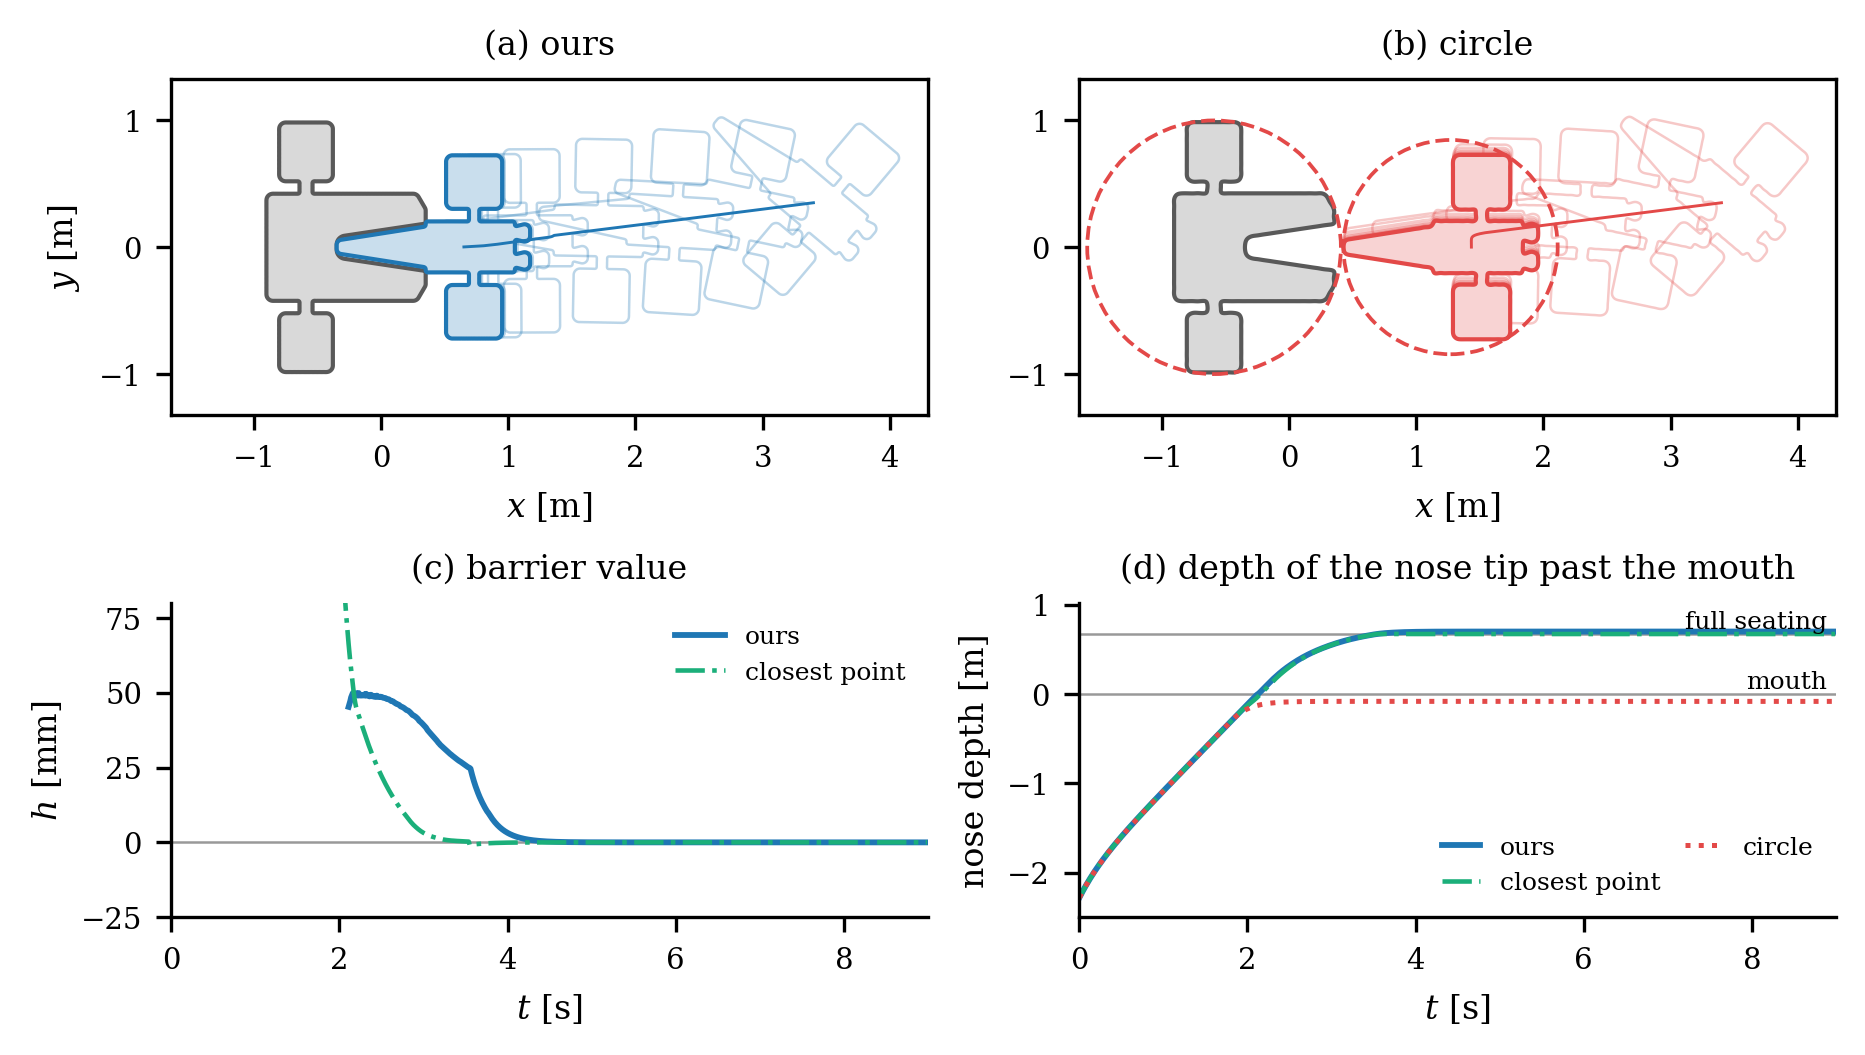
\includegraphics[width=\textwidth]{dock_paper.png}
\caption{Docking into a tapered receptacle with the module fixed. (a) Our barrier (B-spline field):
the vehicle rotates while approaching and seats its 0.70-m nose to within 2~mm of full seating,
with a final ground-truth gap of 32~mm. (b) Minimum enclosing circles (dashed): the vehicle stops
with its nose tip 8~cm in front of the mouth. Poses every 0.6~s; gray: ground truth; colored and
black: certified fitted boundaries. (c) Barrier value: our B-spline field keeps $h\ge0$, the $C^0$
field violates its constraint by 16~mm, and the closest-point barrier by 0.9~mm. (d) Depth of the
nose tip past the mouth (full seating: 0.668~m).}
\label{fig:dock}
\end{figure*}

\begin{table}[t]
\caption{Docking into a Tapered Receptacle with Different Barriers}
\label{tab:dock-base}
\centering
\footnotesize
\setlength{\tabcolsep}{2.6pt}
\renewcommand{\arraystretch}{1.05}
\begin{tabular}{lccccc}
\toprule
& \multicolumn{3}{c}{ours} & closest & \\
\cmidrule(lr){2-4}
& B-spline & B\'ezier & B\'ezier & point & circle\\
\midrule
cells & $82^2{\times}384$ & $30^3$ & $46^3$ & -- & --\\
coefficients [$10^6$] & 2.77 & 0.75 & 2.67 & -- & --\\
certified $l^\star$ [mm] & \textbf{12.3} & 19.0 & 16.2 & -- & --\\
nose depth [m] & 0.666 & 0.692 & 0.689 & 0.671 & $-0.084$\\
min.\ true gap [mm] & 24.8 & 6.1 & 9.4 & 28.4 & 102.5\\
min.\ $h$ [mm] & \textbf{0.0} & $-15.8$ & $-9.6$ & $-0.9$ & --\\
input total variation & 3.6 & 161 & 94.5 & 3.8 & 2.5\\
time per step [ms] & 0.61 & 0.52 & -- & 6.82 & 0.25\\
\bottomrule
\end{tabular}
\\[3pt]
\parbox{\columnwidth}{\footnotesize Nose depth: tip position past the mouth at the end (full
seating 0.668~m). Time per step: median, complete filter. The circle barrier's $h$ is in m$^2$ and
stayed nonnegative.}
\end{table}

Our B-spline barrier docks smoothly while respecting its constraint (Table~\ref{tab:dock-base}): the
nose stops 2~mm short of full seating at $h=0$, with a final ground-truth gap of 32~mm, i.e., the
boundary offsets, the certified level, and the remaining error of the field at this configuration.
Both $C^0$ piecewise B\'ezier fields push the nose deeper only by violating their own constraints by
15.8 and 9.6~mm; the one with a matched number of coefficients is certified at a lower level but
still violates, and in both, the constraint normal switches across cell faces and the input chatters
(total variations 161 and 94.5, against 3.6 for ours). Their true shapes do not touch only because
of the boundary offsets. On this geometry, the closest-point barrier docks as smoothly as ours, with
a violation of 0.9~mm, because the contact stays on the tapered walls and the closest pair does not
jump; it costs 11 times more per step. The minimum enclosing circles stop the vehicle with its nose
tip 8~cm in front of the mouth.

\emph{Time step.} Refining the time step from 10 to 1~ms leaves our barrier nonnegative and the final
pose unchanged to the micrometer. The violation of the $C^0$ field stays between 15.1 and 15.8~mm,
while its input total variation grows from 161 to 1521, i.e., it chatters at the sampling rate; the
violation of the closest-point barrier shrinks from 0.9 to below $10^{-3}$~mm. The violation of the
$C^0$ field is therefore caused by its gradient jumps rather than by the discretization, whereas that
of the closest-point barrier here is a discretization effect.

\emph{Angular resolution.} With 96, 192, and 384 angular cells, the certified level is 12.4, 12.1,
and 12.3~mm, but the nose stops 1.5, 0.1, and 0.2~cm short of full seating. The free configurations
near full seating form a narrow ridge in $\theta$; coarse angular cells round it off, so the field
underestimates the distance there and stops the vehicle early, even though the certified level
hardly changes. Near a tight fit, the relevant measure of conservatism is therefore the attainable
insertion rather than $l^\star$ alone.

\subsection{Five Robots with Random Non-Convex Shapes}\label{sec:exp-five}
Five shapes are generated as star-shaped radial Fourier series with a hull-area ratio below 0.9,
scaled to radii of 0.85--1.08~m, and sampled as polygons with 400 vertices, which serve as the
ground truth. Each is enclosed by a certified B-spline boundary (Sec.~\ref{sec:cert-body}) with 24
control points and outward offsets of 8--20~mm. For the ten pairs, fields with about 6-cm cells are
fitted and certified in 11--16~s per pair; the certified levels are 17--26~mm, and the activation
band (minimum field value 0.13--0.29~m) and regularity are certified for all pairs. The robots are unicycles ($|v|\le1$~m/s, $|\omega|\le\pi/2$~rad/s)
with the barrier derivative~\eqref{eq:hdot-uni}, and each moves to the position two places over on
a circle of radius 4~m, so that the five paths cross in a star pattern. With exactly antipodal
goals, all paths meet at the center and the unicycles block each other there, and we do not resolve
such deadlocks~\cite{reis2020undesirable}; we therefore use the star pattern and perturb the start
and goal angles on the circle by up to $9^\circ$ and $20^\circ$, respectively. All robots reach
their goals after 10.0~s (Fig.~\ref{fig:five}); the minimum distance between ground-truth shapes
over all pairs is 23.0~mm, and the minimum active $h$ is $-1.1$~mm, a discrete-time effect
(Sec.~\ref{sec:exp-stats}).

\begin{figure}[t]
\centering
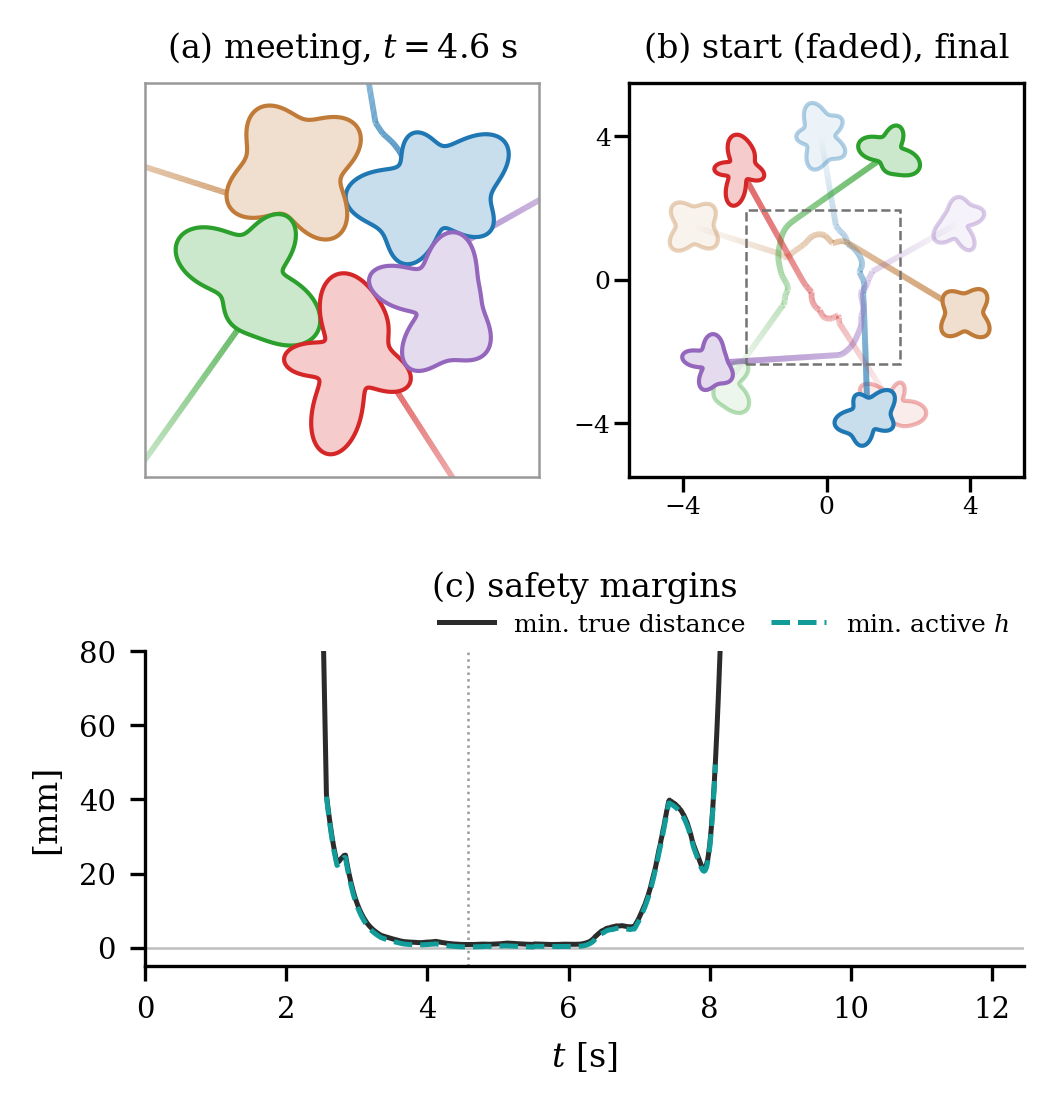
\includegraphics[width=0.92\columnwidth]{five_paper.png}
\caption{Five unicycle robots with random non-convex shapes exchanging positions on a circle in a star
pattern (gray: ground truth; colored: certified fitted boundaries). (a) Start poses (faded), final
poses, which coincide with the goals, and robot-center paths. (b) Minimum ground-truth distance over
all pairs and minimum barrier value over active pairs.}
\label{fig:five}
\end{figure}

\subsection{Random Swaps: Comparison with Baselines}\label{sec:exp-stats}
Using the same five random shapes at half the size (radii 0.43--0.54~m, offsets 4--12~mm, certified
levels 15--23~mm), we draw 20 random instances with start and goal poses uniformly in
$[-3,3]^2\times\Sone$ (pairwise center distances at least $\rho_i+\rho_j+0.5$~m) and run all three
barriers for 15~s (Table~\ref{tab:stats}).

\begin{table}[t]
\caption{Twenty Random Five-Robot Instances}
\label{tab:stats}
\centering
\footnotesize
\setlength{\tabcolsep}{5pt}
\renewcommand{\arraystretch}{1.05}
\begin{tabular}{lccc}
\toprule
& ours & closest point & circle\\
\midrule
instances with a collision & \textbf{0} & 5 & \textbf{0}\\
min.\ ground-truth distance [mm] & $+19.7$ & $-86.8$ & $+42.7$\\
min.\ $h$ [mm] & $-2.4$ & $-114.4$ & --\\
instances with $\min h<-0.01$~mm & 8 & 11 & 0\\
instances with all goals reached & 13 & 12 & \textbf{20}\\
\quad of which collision-free & 13 & 11 & \textbf{20}\\
time to goals$^\ast$ [s] & 6.19 & 6.18 & 6.32\\
path length$^\ast$ [m] & 15.80 & 15.82 & 15.82\\
time per step, median [ms] & 0.66 & 2.74 & 0.40\\
time per step, max.\ [ms] & 16.3 & 30.2 & 1.5\\
steps requiring slack & 0 & 0 & 0\\
\bottomrule
\end{tabular}
\\[3pt]
\parbox{\columnwidth}{\footnotesize $^\ast$Mean over the 11 instances completed without collision by
all three barriers. Horizon 15~s, time step 10~ms. Negative distances: depth of the deepest vertex
inside the other polygon. The circle barrier's $h$ is in m$^2$ and stayed nonnegative.}
\end{table}

The closest-point barrier collides in 5 of 20 instances, with vertices up to 87~mm inside the other
body; one of these instances nevertheless reaches all goals. In our single-closest-pair
implementation, the closest pair of non-convex bodies jumps, the barrier derivative is only
one-sided, and the constraint normal can point the wrong way just before contact; feature switches,
the polygonal sampling of the boundaries, and the 10-ms time step all contribute, and we cannot
separate them. These results therefore concern this closest-point construction, the one analyzed
in~\cite{jo2026geometry}, and not nonsmooth formulations that account for all active closest
features. Our barrier and the circles never collide. The circles, however, reach all goals, whereas
ours reaches them in 13 instances and ends in a deadlock in 7: round surrogates slide past each
other, while exact non-convex boundaries can hook and block each other, and we do not resolve
deadlocks. On the 11 instances completed without collision by all methods, times and path lengths
differ by less than 3\%; in this open, uncluttered setting, the conservatism of circles costs little.
The benefit of exact geometry appears in tight interactions such as docking
(Table~\ref{tab:dock-base}), where circles cannot complete the task. Over all instances, our barrier
keeps a minimum ground-truth distance of 19.7~mm, against 42.7~mm for the circles, whose clearance is
dictated by the enclosing radii rather than by the geometry.

The continuous-time guarantee does not carry over exactly to the sampled controller: in 8 of the 20
instances, our barrier dips below $-0.01$~mm, by at most 2.4~mm, when several pairs are active and
the robots move at full speed; the ground-truth distance nevertheless stays above 19.7~mm, owing to
the certified level and the boundary offsets. A sampled-data tightening of~\eqref{eq:qp} would be
needed to make the guarantee hold for the implemented controller (Sec.~\ref{sec:limits}).

\subsection{Unicycle Robots}\label{sec:exp-unicycle}
We repeat the position swaps of~\cite{jo2026geometry} with unicycle dynamics ($|v|\le1$~m/s,
$|\omega|\le\pi/2$~rad/s) and the barrier derivative~\eqref{eq:hdot-uni}; the nominal controller steers
toward the goal position. For the C-shape and the three-lobed body swapping along a line with lateral
offset $d_y\in\{0,0.1,\dots,0.6\}$~m, no instance collides (minimum ground-truth distance
10.6--22.4~mm). For $d_y\le0.4$~m, the robots end in a deadlock; for $d_y=0.5$~m, the barrier is active
(minimum $h=1.0$~mm) and both robots reach their goals after 7.8~s; for
$d_y=0.6$~m, they pass without interaction. For four heterogeneous robots at the corners of squares
with half-sides of 0.9--2.2~m, diagonal swaps never collide (minimum distance 20.1~mm) but always
deadlock at the center, whereas moves to the neighboring corner complete without interaction. In all
unicycle runs, the norm of the input coefficient vector of the barrier stays above 0.128 (two robots)
and 0.684 (four robots) whenever $h<0.05$~m, so no loss of relative degree occurs, and no step
requires slack. The five-robot experiment of Sec.~\ref{sec:exp-five} also uses unicycle dynamics.
\subsection{One Field for Many Static Obstacles}\label{sec:exp-static}
Following Remark~\ref{rem:static}, a robot (random shape 0) moves through a $7.6\times7.6$~m
workspace with $m\in\{1,3,5,7\}$ random non-convex obstacles, each enclosed by a certified B-spline
boundary, along waypoints whose horizontal legs pass the middle row of obstacles at 0.6~m, while
rotating by $90^\circ$ per leg. One field of $122\times122\times48$ cells
($7.1\times10^5$ coefficients) encodes all obstacles (Table~\ref{tab:static}). To keep the larger
raster affordable, its training targets use a 2-cm raster, which, by Sec.~\ref{sec:exp-sens},
explains the larger certified levels (39--41~mm).

\begin{table}[t]
\caption{Robot among $m$ Static Obstacles}
\label{tab:static}
\centering
\footnotesize
\setlength{\tabcolsep}{5pt}
\renewcommand{\arraystretch}{1.05}
\begin{tabular}{lcccc}
\toprule
$m$ & 1 & 3 & 5 & 7\\
\midrule
certified $l^\star$ [mm] & 39.4 & 40.9 & 40.9 & 40.9\\
certification time [s] & 1.3 & 2.4 & 3.7 & 5.0\\
band / regularity certified & yes & yes & yes & yes\\
min.\ true distance, ours [mm] & 959 & 951 & 37 & 36\\
time per step, ours, median [ms] & 0.37 & 0.37 & 0.42 & 0.45\\
time per step, closest pt., median [ms] & 0.20 & 0.20 & 2.62 & 2.78\\
time per step, closest pt., max.\ [ms] & 0.52 & 0.60 & 8.06 & 7.40\\
\bottomrule
\end{tabular}
\\[3pt]
\parbox{\columnwidth}{\footnotesize Ours: one field for all obstacles. Closest point: one
constraint per obstacle within reach.}
\end{table}

All runs reach the final pose without collision. With 5 and 7 obstacles, the barrier is active
(minimum $h=1.2$~mm, ground-truth clearance 36~mm); with 1 and 3 obstacles, none lies near the path.
The online cost of our filter is one field evaluation and stays at 0.37--0.45~ms regardless of $m$,
whereas the closest-point baseline needs one distance computation per nearby obstacle and grows to
2.8~ms (median) and 7.4~ms (maximum) with seven obstacles. The offline cost grows with the workspace:
fitting takes about 35~s, and certification grows mildly with the total boundary length, from 1.3 to
5.0~s.

The curved-maze escape experiment uses a single winding passage (Fig.~\ref{fig:static}). It is
derived from a manually traced maze: the passage from the upper-left entrance to the lower-right
exit is kept, its blind branches are removed, and the passage is smoothed into a tube whose
centerline and width vary smoothly along its length. The two resulting non-convex wall regions,
bounded by smooth closed curves, form the physical ground truth. Each is enclosed by a separately
fitted periodic cubic B-spline with nonuniform knots (6319 and 6661 control points), using a 1-mm
outward fitting offset; the computed maximum distance from each fitted curve to its physical wall
boundary is bounded by 1.41~mm, including curve sampling and reference chord-error bounds.
Subdivision verifies that every fitted control hull stays outside the reference polygon by more
than its chord-error bound; a winding test establishes enclosure of each wall. The robot is a
rocket-shaped body with a nose, a fuselage, and two side fins, 0.54~m long and 0.30~m wide,
enclosed by a certified periodic B-spline boundary with 64 control points and a 4-mm offset. A
single $160\times160\times48$-cell field ($1.3\times10^6$ coefficients) encodes both fitted walls
for the rocket; contact, boundary-band, and regularity checks pass, with $l^\star=45.5$~mm (contact
certificate in 56~s). The nominal controller only moves toward nine goal waypoints: from an offline
route, we keep the fewest route points whose connecting segments enter the walls by at most 10~cm,
so the straight segments cut the corners and the barrier, not the waypoints, keeps the rocket off
the walls. The input bounds are $v_{\max}=0.8$~m/s and $\omega_{\max}=1.4$~rad/s, with a 10-ms
step. The rocket reaches the exit in 39.8~s along a 28.0-m path while sliding along the walls: the
barrier modifies the nominal input in 2975 of the 3984 steps (75\%). The minimum sampled clearance
to the physical walls is 26.8~mm; wall distances use polygonal approximations with a uniform
chord-deviation bound below 0.1~mm, which is subtracted from the measured separation, and a
rigid-motion bound verifies a clearance of at least 22.5~mm over every integration interval, with
no unresolved interval. The minimum sampled barrier value is $-1.1$~mm, a discrete-time effect as in
Sec.~\ref{sec:exp-stats}, and the median online cost is 0.5~ms. These maze measurements are
distinct from the obstacle-count study in Table~\ref{tab:static}.

\begin{figure}[t]
\centering
\includegraphics[width=\columnwidth]{rocket_maze.pdf}
\caption{Escape of a rocket-shaped robot through a curved maze with a single configuration-space
field and nine goal waypoints. Gray with red outlines: maze walls (ground truth and certified fitted
boundaries); gray with blue outlines: rocket (ground truth and certified fitted boundary) at
intermediate poses; blue line: trajectory of the rocket's reference point.}
\label{fig:static}
\end{figure}

% -----------------------------------------------------------------------------
% Fixed-orientation diagnostic, independently implemented adapted baselines.
\subsection{Comparison on a Shared Configuration-Space Envelope}
\label{sec:three-baselines}
We compare the proposed field with adaptations of the sampling-based nonsmooth
barrier of Lutkus et al.~\cite{lutkus2025sampling} and the deforming ball-world
controller of Notomista and Saveriano~\cite{notomista2021nonconvex}.
To isolate online representation and control costs, all methods receive the same
smooth conservative configuration-space envelope for a fixed-orientation
non-convex cross-shaped robot translating past one non-convex cross-shaped
obstacle. The exact configuration obstacle is a union of four rectangles; a
periodic radial spline encloses its 20-mm clearance dilation, with a continuous
containment bound obtained from angular Lipschitz constants.
This shared-envelope experiment does not compare the methods' complete geometry
preprocessing pipelines or their performance under rotation.

Our constant-orientation field reduces exactly to a bicubic B-spline, whose
boundary level, activation band, and regularity are verified offline.
The sampling baseline uses $N\in\{64,256,1024\}$ boundary samples and a
covering-radius correction. It enforces all sample constraints that are not
redundant under the input bound, including all active minimizers, rather than
selecting one closest feature. The ball-world baseline uses the single-obstacle
radial diffeomorphism $F(x)=q_c+\rho(x-c)/r(\arg(x-c))$, and controls both
$q_c$ and $\rho$. Its implementation includes the derivative with respect to
the changing map parameters and joint rate scaling for the physical speed
bound. These are independent adaptations, not reproductions of the source
papers' experimental setups.

Six offset approaches share the nominal controller, a 0.6-m/s input bound,
gain 5, a 10-ms step, and a 12-s horizon. We evaluate physical-body separation,
online computation, and input total variation; goal completion and deadlock
resolution are outside this comparison. A common interval motion bound checks
the 20-mm clearance along the linearly interpolated translation trajectories,
with explicit unresolved intervals. Online timings are additionally measured
at identical physical states to separate query cost from trajectory differences.
The arithmetic uses double precision without verified rounding bounds.

% Generated by compare_three_baselines.py from results/three_baselines/comparison.json.
\begin{table}[t]
\caption{Shared Configuration-Space Benchmark (Six Fixed-Horizon Runs)}
\label{tab:three-baselines}
\centering\footnotesize
\setlength{\tabcolsep}{3pt}
\begin{tabular}{lrrrr}
\toprule
Method & median & p95 & min. gap & input TV\\
 & [ms] & [ms] & [mm] & [m/s]\\
\midrule
Ours & 0.106 & 0.161 & 29.4 & 0.89 \\
Samples, $N=64$ & 0.159 & 0.247 & 118.8 & 1.07 \\
Samples, $N=256$ & 0.164 & 0.259 & 40.0 & 0.85 \\
Samples, $N=1024$ & 0.207 & 0.308 & 29.3 & 0.78 \\
Ball world (adapted) & 0.217 & 0.336 & 22.1 & 8.57 \\
\bottomrule
\end{tabular}
\\[3pt]
\parbox{\columnwidth}{\footnotesize Times: identical pose queries, complete CPU
controller including the QP; ball-world state reset before each timed query.
Gap: minimum evaluated physical-body separation over the six closed-loop runs.
Input TV: mean $\sum_k\|v_{k+1}-v_k\|_2$ over the fixed 12-s horizon.
No collision or unresolved clearance interval occurred for any method.}
\end{table}

Table~\ref{tab:three-baselines} shows the sampling resolution--clearance tradeoff.
The field and the fine-sampling baseline achieve similar minimum physical gaps;
the comparison reports their measured cost without assuming that smoothness
alone guarantees lower input variation. The ball-world result measures its
deforming-map overhead and physical safety in this shared geometry, without
ranking its progress behavior. These measurements are specific to the present
implementation and single-obstacle benchmark.

\section{Limitations}\label{sec:limits}
\emph{Scope of the certificate.} The certificate excludes first contacts; it does not show that the
whole configuration-space obstacle lies below the level (Sec.~\ref{sec:cert}), so it protects only
trajectories that start collision-free. It certifies non-intersection, not a prescribed clearance.
Because the level absorbs the largest overestimate of the field on $\Mset_{ij}$, contact could in
principle be approached where the field is least accurate. In all our runs with the B-spline field,
the ground-truth distance stayed above 10.6~mm, owing to the outward offsets of the fitted
boundaries and to the level. A clearance $c>0$ can be certified by enclosing the dilated ground truth
$\mathcal G_i\oplus\{\norm{\mathbf y}\le c/2\}$ instead of $\mathcal G_i$, i.e., by requiring every
control hull of the boundary curve to keep a distance of at least $c/2$ from $\mathcal G_i$.

\emph{Discrete time.} All guarantees hold in continuous time. With a 10-ms time step, the B-spline
barrier dipped to $-2.4$~mm in random five-robot swaps (Sec.~\ref{sec:exp-stats}), and the
closest-point barrier violated its constraint by up to 114~mm; the $C^0$ field violated its
constraint by about 15~mm in docking at every time step down to 1~ms (Sec.~\ref{sec:exp-probe}). A sampled-data tightening
of~\eqref{eq:qp}, e.g., with a margin derived from Lipschitz bounds of the field, which the Bernstein
coefficients of its derivatives provide, is needed for a guarantee of the implemented controller.

\emph{Arithmetic.} The certificates are computed in double precision without outward rounding
(Sec.~\ref{sec:cert}); a verified implementation needs interval arithmetic.

\emph{Deadlock and liveness.} Proposition~\ref{prop:feas} guarantees feasibility on the safe set but
not progress. Exact non-convex geometry makes mutual blocking more frequent than with round
surrogates (7 of 20 random instances and the four-robot diagonal unicycle swaps).
Deadlock resolution is not addressed.

\emph{Training data.} Beyond moderate model sizes, the conservatism is set by the accuracy of the
training targets; our rasterized targets overestimate distances by about one raster cell.

\emph{Dimension and offline cost.} The field lives in the configuration space of the pair. For
planar bodies, this space is three-dimensional; spatial bodies with full rotation require six
dimensions, where tensor-product fields are impractical (about $6\times10^7$ coefficients at 20 per
axis). Translation-only and yaw-only spatial settings (three and four dimensions) remain tractable.
Heterogeneous teams with $K$ shape types need $K(K+1)/2$ fields.

\emph{Evaluation.} The rotating-body experiments compare against a single-closest-pair workspace
barrier and bounding circles. Section~\ref{sec:three-baselines} adds adapted sampling-based and
ball-world controllers on shared fixed-orientation geometry; it does not establish performance
under rotation or across different geometry preprocessing pipelines. Polytopic
barriers~\cite{chen2025minkowski,chen2026exact,thirugnanam2025strongly}, which require convex
decompositions of the non-convex bodies, remain to be compared. The random-shape study uses one set
of five shapes and 20 instances, and all experiments are in simulation.

% -----------------------------------------------------------------------------
\section{Conclusion}\label{sec:concl}
We extended geometry-aware CBFs from workspace SDFs evaluated at closest points to
configuration-space SDFs over the full planar pose. A single smooth B-spline field per pair of
bodies, or per robot for any number of static obstacles, yields one scalar barrier for non-convex
rotating shapes. A first-contact lemma reduces collision avoidance to a bound on an explicit
three-parameter set, which a Bernstein branch-and-bound certifies without constructing
configuration-space obstacles; the same machinery certifies the activation band and the regularity
of the barrier, and the filter is feasible wherever all barriers are nonnegative. Within a common
Bernstein-form family, the $C^2$ B-spline is both more accurate than the global polynomial
of~\cite{jo2026geometry} and free of the chattering caused by $C^0$ patches. In simulation, the
barrier never produced a collision, unlike a closest-point barrier, reached deeper into concavities
than bounding circles, and kept a constant online cost as obstacles were added. Its conservatism is
concentrated in a few cells and is currently limited by the training data, which points to
spatially varying levels and exact training targets as next steps, together with verified
arithmetic, sampled-data guarantees, deadlock resolution, and hardware validation.

\bibliographystyle{IEEEtran}
\bibliography{references}

\end{document}
